\begin{figure}
\begin{center}
    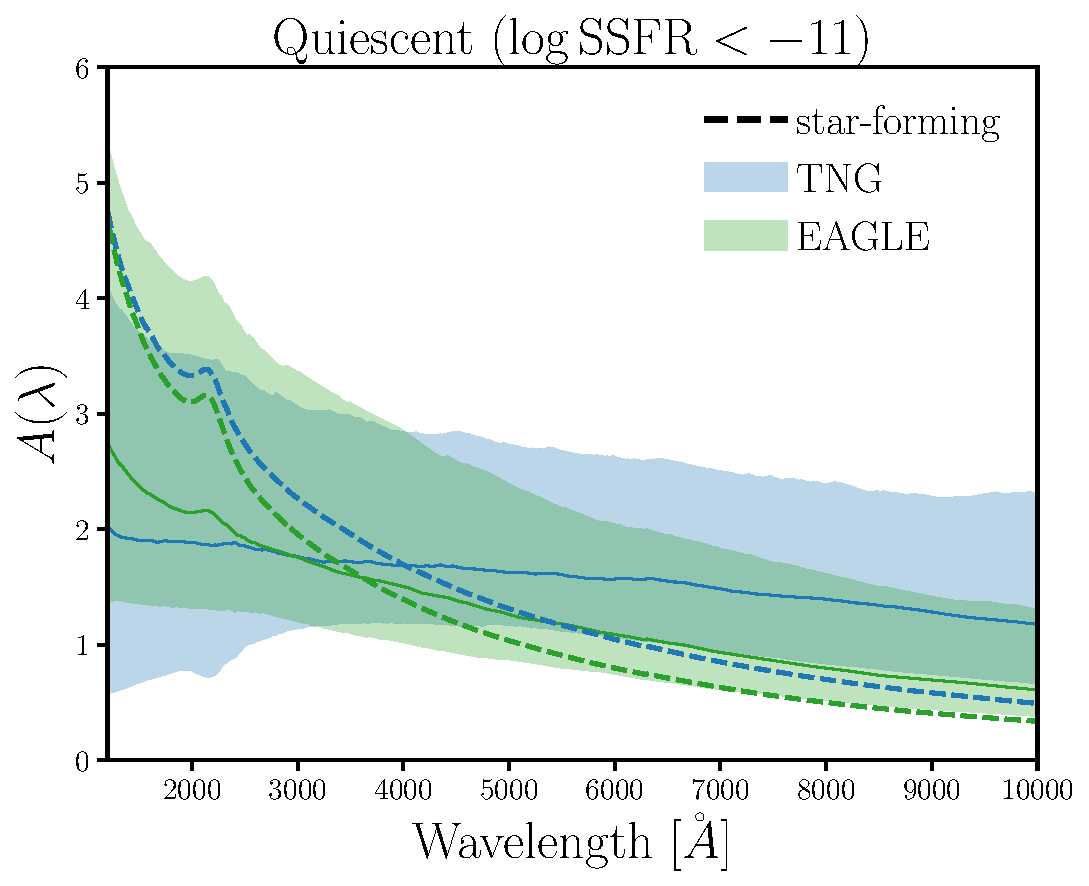
\includegraphics[width=0.9\textwidth]{figs/abc_q_atten_unnorm.pdf}
    \caption{\label{fig:q_raw_atten}
    The attenuation curves of quiescent galaxies predicted by the \eda~for
    median posterior parameter values of SIMBA (left), TNG (center), and
    EAGLE (right).
    Galaxies with $\ssfr < 10^{-11}yr^{-1}$are classified as quiescent.
    We mark the 68 percentile of the attenuation curves with the shaded region
    and include the predicted attenuation curves of star-forming galaxies for
    comparison (dashed). 
    In all three simulations, \emph{the \eda~predicts attenuation curves that
    have lower amplitudes and shallower slopes than star-forming galaxies.}
    }
\end{center}
\end{figure}
\subsection{The Attenuation Curves of Quiescent Galaxies}  
%We have demonstrated so far that the \eda~can reproduce the observed UV and optical color-magnitude relations.  
%In doing so, it also predicts attenuation-slope relation and dust attenuation curves of star-forming galaxies that are in good agreement with observations and radiative transfer simulations. 
In addition to star-forming galaxies, the \eda~also makes predictions on the
dust attenuation of quiescent galaxies. 
This is particularly valuable since dust attenuation in quiescent galaxies is
still poorly constrained by observations due to challenges in directly
measuring it from observations. 
For instance, methods that rely on IR luminosities can be contaminated by MIR
emission from AGN heating nearby dust~\citep{kirkpatrick2015}. 
SED fitting methods must also account for AGN MIR
emission~\citep{salim2016, leja2018, salim2018} and struggle to tightly
constrain dust attenuation for quiescent galaxies due to the degeneracies
with star formation history and metallicity.
With a forward modeling approach, we circumvent these challenges. 
Instead, we derive the attenuation curves necessary for the simulated quiescent
population to reproduce the observed optical and UV photometry. 

In Figure~\ref{fig:q_raw_atten}, we present the attenuation curves of
quiescent galaxies predicted by the \eda~for the median posterior parameter
values of SIMBA (left), TNG (center), and EAGLE (right). 
Quiescent galaxies are classified using a $\ssfr < 10^{-11}{yr}^{-1}$ cut. 
Unlike Figure~\ref{fig:sfatten}, we do not normalize the attenuation curves at
$3000\AA$.  
For comparison, we include $A(\lambda)$ of star-forming galaxies predicted
by the \eda~for the corresponding simulation in each panel (dotted).
In all three simulations, quiescent galaxies have attenuation curves with
overall lower amplitudes and shallower slopes than star forming galaxies.

We predict $A(\lambda)$ with lower amplitude for quiescent galaxies because
quiescent galaxies in SIMBA, TNG, and EAGLE without dust are only slightly
more luminous than observations. 
In the top panels of Figure~\ref{fig:obs}, we see that the most luminous
galaxies with the highest $\gr$ color is $<0.5~mag$ brighter than the tip of
the red sequence in the SDSS color-magnitude relation. 
For SIMBA+\eda, where we predict $A(\lambda) \sim 0$, the most luminous and
optically red galaxies have comparable $M_r$ as the tip of the SDSS red sequence.
In contrast, the most luminous blue, star-forming, galaxies are $>1~mag$
brighter than the luminous end of the SDSS blue cloud.
Despite having lower attenuation than star-forming galaxies, in TNG and
EAGLE we predict significant dust attenuation in quiescent galaxies, $A_V > 0.5$.
\chedit{
    Although this could be a due to shortcomings in TNG and EAGLE in producing
    quiescent galaxies that are intrinsically too luminous, the prescence of
    dust attenuation in quiescent galaxies, which is typically neglected, has
    significant implications.  
}
For instance, it strengthens the evidence for the UV upturn phenomenon, the
unexpected detections of UV flux in quiescent galaxies~\citep[\eg][]{code1969,
oconnell1999, lecras2016, ali2018, dantas2021}. 
Constraints on the attenuation in quiescent galaxies may also help discern
among the different hypotheses: residual star formation
activity~\citep[\eg~][]{kaviraj2007}, post-main-sequence stellar evolutionary
phases~\citep[\eg~][]{yi1997}, or binary systems~\citep[\eg~][]{han2007}.
Since the attenuation curves of quiescent galaxies are difficult to measure
from observations, the \eda~predictions highlight the advantages of a
forward modeling approach and its complementarity with standard approaches. 

In Figure~\ref{fig:q_raw_atten}, we also find that quiescent galaxies have
shallower attenuation curves than star-forming galaxies. 
This is a consequence of the fact that SIMBA, TNG, and EAGLE all predict
intrinsically UV-red galaxies that do not require significant reddening by
dust. 
This is especially true for SIMBA and TNG, which predict significant
number of galaxies with intrinsic $\fnuv > 1$ (Figure~\ref{fig:obs}
and~\ref{fig:uv_sfh}).
These galaxies are quiescent ($\ssfr < 10^{-11}yr^{-1}$) and have high
$\fnuv$ due to a lack of recent star formation contributing to the
SED~\citep{leja2017}. 
When we examine their SFHs, we find that, although they have more star
formation than the luminous UV-red galaxies we discuss earlier, they have
little star formation in the last 1 Gyr. 
This implies that SIMBA, whose quiescent galaxies have the shallowest
attenuation curve, has the most efficient star-formation quenching among
the simulations. 

The mass resolution of the simulations can impact the SFHs of quiescent
galaxies and, thus, can also impact their observables.
The SFHs of simulated galaxies cannot include any star formation below the
resolution limit, so the SEDs we compute from them do not include any star
formation below the mass resolution. 
For recent star formation, this can significantly impact on the SED,
especially in the FUV and NUV wavelength ranges~\citep{leja2017}. 
SIMBA, in particular, has a significantly higher mass resolution
($1.82\times10^7M_\odot$) than TNG or EAGLE ($1.4\times10^{6}M_\odot$,
$1.81\times10^6M_\odot$).
Fortunately, the quiescent galaxies that pass the $M_r$ and UV selection
in our forward model have $M_* \gtrsim 10^{10}M_\odot$ (see
Figure~\ref{fig:avmsfr} later). 
\chedit{
    Even if we were to include in their SFHs a $< 100{\rm Myr}$ old stellar
    population, with total mass equivalent to the mass resolution limit, the
    impact on $\fnuv$ would be small: $<0.1~mag$ for SIMBA and $\lesssim
    0.01~mag$ for TNG and EAGLE.
}
Hence, mass resolution does not significantly impact the dust attenuation
we predict for quiescent galaxies.  

Despite the advantages of our forward modeling approach in deriving dust
attenuation curves for quiescent galaxies, we caution readers
that we only vary the \eda~parameters in this work.     
The \eda~predictions of the quiescent galaxy dust attenuation described in this
section assumes that the simulations accurately model the star formation and
metallicity histories of quiescent galaxies. 
Shortcomings in the galaxy formation models, and not the dust attenuation, may
be responsible for the intrinsic differences between the quiescent populations
in simulations and observations. 
For instance, we already find in Section~\ref{sec:results} that quenching
is too efficient in certain SIMBA and TNG quiescent galaxies and results
in luminous UV-red galaxies not found in SDSS. %that cannot be reconciled by dust attenuation. 
TNG and EAGLE may also be producing quiescent galaxies that are
overall intrinsically too luminous, which then requires significant dust
attenuation to match observations.
In principle, however, we can vary both the \eda~parameters and the parameters
of the galaxy formation models and infer them simultaneously with a foward
modeling approach. 
We will explore this in future work. 
